\documentclass{osa-article}

%% Select the journal you're submitting to
%% oe, boe, ome, osac, osajournal
\journal{osajournal}
% Key:
% Express journals must have the correct journal selected:
% {oe} Optics Express
% {boe} Biomedical Optics Express
% {ome} Optical Material Express
% {osac} OSAC Continuum
% Other OSA journals may use:
% {osajournal} Applied Optics, Advances in Optics and Photonics, Journal of the Optical Society of America A/B, Optics Letters, Optica, Photonics Research

% Uncomment if submitting to Photonics Research.
% ONLY APPLICABLE FOR \journal{osajournal}
% \setprjcopyright

% Set the article type
\articletype{Research Article}
% Note that article type is not required for Express journals (OE, BOE, OME and OSAC)

% Talon's custom libraries
\usepackage{empheq}
% \usepackage{bm}

% Talon's custom commands
\newcommand{\argmin}{\arg\!\min}
\newcommand{\me}{\mathrm{e}}
\providecommand{\e}[1]{\ensuremath{\times 10^{#1}}} 
\providecommand{\mb}[1]{\mathbf{#1}}
\providecommand{\mf}[1]{\mathfrak{#1}}
\providecommand{\mc}[1]{\mathcal{#1}}
\providecommand{\ro}{\mathbf{\mathbf{r}}_o}
\providecommand{\so}{\mathbf{\hat{s}}_o}
\providecommand{\rb}{\mathbf{r}_b}
\providecommand{\rbm}[1]{r_b^{\text{m}}}
\providecommand{\rd}{\mathbf{r}_d}
\providecommand{\rdf}{\mathpzc{r}_d}
\providecommand{\mh}[1]{\mathbf{\hat{#1}}}
\providecommand{\mbb}[1]{\mathbb{#1}}
\providecommand{\bs}[1]{\boldsymbol{#1}}
\providecommand{\bv}{\bs{\nu}}
\providecommand{\bsh}[1]{\hat{\boldsymbol{#1}}}
\providecommand{\nan}{\left(\frac{\text{NA}}{n_o}\right)}
\providecommand{\lmsum}{\sum_{\ell=0}^\infty\sum_{m=-\ell}^{\ell}}
\providecommand{\intr}[1]{\int_{\mbb{R}^{#1}}}
\providecommand{\ints}[1]{\int_{\mbb{S}^{#1}}}
\providecommand{\tb}[1]{\textcolor{blue}{#1}}
\DeclareFontFamily{OT1}{pzc}{}
\DeclareFontShape{OT1}{pzc}{m}{it}{<-> s * [1.10] pzcmi7t}{}
\DeclareMathAlphabet{\mathpzc}{OT1}{pzc}{m}{it}
\newcommand{\eqname}[1]{\tag*{#1}}
\newcommand*\widefbox[1]{\fbox{\hspace{1em}#1\hspace{1em}}}

\begin{document}

\title{Spatio-angular fluorescence microscopy I. Basic theory}

\author{Talon Chandler,\authormark{1,*} Author order TBD,\authormark{2,*} and Patrick La Rivi\`ere \authormark{1}}

\address{\authormark{1}University of Chicago, Department of Radiology, Chicago, Illinois 60637, USA\\
\authormark{2}Publications Department, The Optical Society, 2010 Massachusetts Avenue NW, Washington, DC 20036, USA\\
\authormark{3}Currently with the Department of Electronic Journals, The Optical Society, 2010 Massachusetts Avenue NW, Washington, DC 20036, USA}

\email{\authormark{*}talonchandler@talonchandler.com} %% email address is required

%\homepage{talonchandler@talonchandler.com} %% author's URL, if desired

%%%%%%%%%%%%%%%%%%% abstract %%%%%%%%%%%%%%%%
%% [use \begin{abstract*}...\end{abstract*} if exempt from copyright]

\begin{abstract*}
  We introduce the basic elements of a spatio-angular theory of fluorescence
  microscopy. We start by modeling a microscope imaging an ensemble of in-focus
  fluorescent dipoles as a linear Hilbert-space operator with domain
  $\mbb{L}_2(\mbb{R}^2\times\mbb{S}^2)$ and range $\mbb{L}_2(\mbb{R}^2)$, and we
  express the operator in terms of four different sets of object-space basis
  functions. We show that the operator takes a particularly convenient form when
  expressed in a basis of spatial and spherical harmonics---a form we call the
  spatio-angular transfer function (SATF). We demonstrate our formalism by
  analyzing a paraxial single-view fluorescence microscope without using the
  monopole or scalar approximations. We show that this microscope has an angular
  band limit, and we demonstrate the value of the transfer function approach by
  efficiently simulating the imaging process with numerical phantoms. Notably,
  we show that information about the out-of-plane orientation of ensembles of
  in-focus fluorophores is imaged in paraxial widefield fluorescence
  microscopes. We discuss the implications of our analysis for all quantitative
  fluorescence microscopy studies and lay out a path towards a complete theory.
\end{abstract*}

\section{Introduction \tb{needs work}}

Fluorescence microscopes are widely used in the biological sciences for
measuring the distribution of fluorophores throughout a sample [cite]. While an
unprocessed fluorescence micrograph reports the approximate distribution of
fluorophores throughout a sample, all microscopes are diffraction limited
[cite], so the image is a blurred version of the true fluorophore distribution.
Therefore, microscopists who are interested in optimal measurements will perform
a computational restoration to recover some of the information lost during the
imaging process.

Restoration techniques attempt to recover the true distribution of fluorophores
using the measured data and a model of the imaging process. A model of the
imaging process can be obtained theoretically (by mathematically modeling the
instrument under idealized conditions), experimentally (by measuring the
instrument's response to a known input), or by a combination of theory and
experiment (by measuring parameters of an instrument model). In all cases the
accuracy of the restored fluorophore distribution is limited by the accuracy of
the imaging model. All theoretical imaging models make simplifying
approximations that limit the accuracy of restorations, so it is important to
verify that the approximations introduce an acceptable level of error. This work
investigates the errors introduced by two common approximations in models of
fluorescence microscopes---the \textit{monopole approximation} and the
\textit{scalar approximation}.

This work lies at the intersection of three classes of fluorescence microscopy:
(1) single-molecule localization microscopy (SMLM), (2) spatial ensemble
fluorescence microscopy including widefield, confocal, and light-sheet
techniques, and (3) polarized fluorescence microscopy. We briefly review these
three classes and focus on their restoration techniques and use of the monopole
and scalar approximations.

The SMLM community has pioneered the use of rigorous electromagnetic models of
fluorescence microscopes \cite{backer2014, lieb2004} [cite Novotny]. When a
single molecule is fluorescing in the sample, the measured intensity pattern is
strongly dependent on the orientation of the emitting molecule. Backlund and Lew
\cite{backlund2014} have shown that ignoring the orientation of fluorophores can
bias position estimates, so the most accurate SMLM experiments must jointly
estimate the position and orientation of each molecule.

Meanwhile, most fluorescence microscopists image ensembles of fluorophores and
restore their images without considering the role that the monopole and scalar
approximations play in the restoration process. A typical fluorescence
microscopist is only interested in the spatial distribution of fluorophores, so
they reason that they can ignore the orientation of the emitters.

A smaller community of microscopists is interested in measuring the orientation
of ensembles of fluorophores \cite{mehta2016} [Forkey, Goldman, Moerner,
Oldenbourg]. These techniques typically use polarized illumination or polarized
detection to make multiple measurements of the same object. Current angular
restoration techniques use a model of the dipole excitation and emission
processes [Fourkas] to recover the orientation of fluorophores using pixel-wise
arithmetic, but these techniques do not perform any spatial restoration so they
do not use all of the information available to the microscopist. To our
knowledge no work has been done to model the complete spatio-angular response of
fluorescence microscopes to ensembles of oriented fluorophores.

\tb{Out of date}
In this work we model ensembles of in-focus dipole absorber/emitters using
electromagnetic optics and the paraxial approximation. In section 2 we model the
excitation and detection processes of dipoles, and we define the most important
quantity in this work---the spatio-angular transfer function (SATF). We
calculate the SATF and show that fluorescence microscopes have an angular band
limit. In section 3 we perform simulations and compare our model to traditional
scalar models. In section 4 we discuss the implications of our work for
fluorescence microscopy and lay out a path towards a complete spatio-angular
theory of fluorescence microscopy.

\subsection{Monopole emission vs. dipole emission \tb{not sure where this section should live}}
Consider a single dipole radiator at the origin with its dipole moment oriented
along a direction $\so$. The dipole emitter creates a time-harmonic electric
field at a position $\mb{r}$ far from the dipole proportional to
\begin{align}
  \mb{E}_{\text{ff}}(\mb{r}, \so) \propto \frac{\text{exp}[ik|\mb{r}|]}{|\mb{r}|}\, \mh{r}\times\so\times\mh{r}.\label{eq:dip}
\end{align}
A typical approach to deriving Equation \ref{eq:dip} is to (1) use Maxwell's
equations to derive the inhomogeneous electromagnetic wave equations then (2)
use potentials to solve the wave equations with a dipole source term, then (3)
drop the terms that decay faster than $1/|\mb{r}|$ [cite Jackson, Novotny,
Teich]. Equation~\ref{eq:dip} shows that dipole radiators emit spherical
wavefronts of polarized light with amplitude proportional to $\cos\theta$ where
$\theta$ is the angle between the field point $\mb{r}$ and the dipole axis
$\so$.

Many models of fluorophores approximate the vector field on the left hand side
of Equation \ref{eq:dip} with a scalar field---the \textit{scalar
  approximation}---and drop the orientation dependence on the right hand
side---the \textit{monopole approximation}. The approximated field is given by
\begin{align}
  U_{\text{ff}}(\mb{r}) \propto \frac{\text{exp}[ik|\mb{r}|]}{|\mb{r}|}. \label{eq:mono}
\end{align}
Models that use Equation \ref{eq:mono} as a starting point do not account for
polarization or dipole orientation effects.

\section{Theory \tb{outline is okay, subsections vary, recently moved changes of basis to the front}}
We begin our analysis with the abstract Hilbert space formalism of Barrett and
Myers \cite{barrett2004}. Our first task is to formulate the imaging process as
a mapping between two Hilbert spaces $\mc{H}: \mbb{U} \rightarrow \mbb{V}$ where
$\mbb{U}$ is a set than contains all possible objects, $\mbb{V}$ is a set that
contains all possible datasets, and $\mc{H}$ is a model of the instrument that
maps between these two spaces. We denote (possibly infinite-dimensional)
Hilbert-space vectors in $\mbb{U}$ with $\mb{f}$, Hilbert-space vectors in
$\mbb{V}$ with $\mb{g}$, and the mapping between the spaces with

\begin{align}
  \mb{g} = \mc{H}\mb{f}.
\end{align}

Once we have identified the spaces $\mbb{U}$ and $\mbb{V}$, we can start
expressing the mapping between the spaces in a specific object-space and
data-space basis. In most cases the easiest mapping to find uses a
delta-function basis---we expand object and data space into delta functions then
express the mapping as an integral transform. After finding this mapping we can
start to investigate the same mapping in different bases.

The above discussion is quite abstract, but it is a powerful point of view that
will enable us to draw new conclusions about all fluorescence microscopes. In
Section \ref{sec:monopole} we will demonstrate the formalism by examining a
familiar monopole imaging model, and we will show that the point spread
function and the optical transfer function are mappings between object and data
space expressed in two different bases. In Section \ref{sec:dipole} we will
extend the monopole imaging model to dipoles and examine the mapping in four
different bases. In Section \ref{sec:para} we will examine the mappings for a
more specific case---a paraxial epi-illumination single-view fluorescence
microscope.

\subsection{Monopole imaging in different bases \tb{50\%}}\label{sec:monopole}
We start by considering a microscope that images a field of in-focus monopoles
by recording the irradiance on a two-dimensional detector. We can represent
the object as a function that assigns a real number to each point on a plane,
so we identify object space as $\mbb{U} = \mbb{L}_2(\mbb{R}^2)$. Similarly, we
have a two-dimensional detector that measures a real number at every point on 
a plane, so data space is the same set $\mbb{V} = \mbb{L}_2(\mbb{R}^2)$. Our
first task is complete---we have identified the geometry of object and data
space.

Next, we find and name the representations of our object and data in a
specific basis. In a delta function basis the object can be represented by a
function $f(\ro)$ called the \textit{monopole density}---the number of
monopoles at the two-dimensional position $\ro$ per unit area. Similarly, in a
delta function basis the data can be represented by a function $g(\rd)$ called
the \textit{irradiance}---the power received by a surface at position $\rd$
per unit area. It may seem pedantic to emphasize that these representations
are in a delta function basis, but we highlight this point to make it clear
that the delta function basis is not special---we can choose a different basis
at will.

% We start by considering a field of in-focus monopoles that have been excited by test
% a spatially uniform beam. As the fluorophores relax, they emit scalar waves in
% the form of Equation \ref{eq:mono}. The waves propagate through the microscope
% and we measure the irradiance on a two dimensional detector.

A reasonable starting point is to assume that the relationship between the
object and the data is \textit{linear}---this is usually true in fluorescence
microscopes since fluorophores emit incoherently so a scaled sum of fluorophores
will result in a scaled sum of the irradiance patterns created by the individual
fluorophores. If the mapping is linear we can write the irradiance as the
integral over a field of monopoles weighted by the detector response due to
single monopoles
\begin{align}
g(\rd) = \int_{\mbb{R}^2}d\ro\, h(\rd,\ro)f(\ro), \label{eq:fwdmono}
\end{align}
where $h(\rd{}, \ro{})$ is the kernel of the integral transform. 

Most fluorescence microscopes are (at least approximately) shift-invariant,
which means that shifting the object will result in a corresponding shift of the
data. The mapping between an object and the data in a linear shift-invariant
fluorescence microscope can be written as
\begin{align}
  g(\rd) = \int_{\mbb{R}^2}d\ro\, h(\rd - \ro)f(\ro).  \label{eq:lsi}
\end{align}
When the imaging system is shift invariant the kernel $h(\rd - \ro)$ is usually
called the \textit{point spread function}.

The mapping between the object and the data in linear shift-invariant
microscopes takes a particularly simple form in a spatial harmonic basis. If we
apply the Fourier convolution theorem to Eq. \ref{eq:lsi} we find that
\begin{align}
  G(\bs{\nu}) = H(\bs{\nu})F(\bs{\nu}),\label{eq:freq}
\end{align}
where the \textit{irradiance spectrum} is given by
\begin{align}
  G(\bs{\nu}) = \int_{\mbb{R}^2}d\mb{r}\, g(\mb{r})\, \text{exp}(-2\pi i\mb{r}\cdot\bs{\nu}),
\end{align}
the \textit{optical transfer function} is given by
\begin{align}
  H(\bs{\nu}) = \int_{\mbb{R}^2}d\mb{r}\, h(\mb{r})\, \text{exp}(-2\pi i\mb{r}\cdot\bs{\nu}),
\end{align}
and the \textit{monopole spectrum} is given by
\begin{align}
    F(\bs{\nu}) = \int_{\mbb{R}^2}d\mb{r}\, f(\mb{r})\, \text{exp}(-2\pi i\mb{r}\cdot\bs{\nu}).
\end{align}
Notice that Eqs. \ref{eq:lsi} and \ref{eq:freq} are expressions of the same
mapping between object and data space in different bases. Figure
\ref{fig:monopole-block} summarizes the relationship between object and data
space in both bases.

\begin{figure}
  \centering
  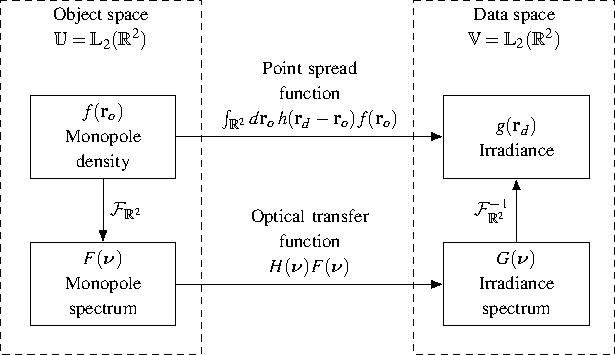
\includegraphics[scale=1.0]{../figures/monopole-block/monopole-block.pdf}
  \caption{We can compute the mapping between object space and data space using
    two different bases.}
     \label{fig:monopole-block}      
\end{figure}

\subsection{Dipole imaging in different bases \tb{50\%}}\label{sec:dipole}
Now we consider a microscope imaging a field of in-focus \textit{dipoles} by
recording the irradiance on a two-dimensional detector. A function that assigns
a real number to each point on a plane is not sufficient to specify a field of
dipoles because the dipoles can have different orientations. To represent the
object we need to extend object space to
$\mbb{U} = \mbb{L}_2(\mbb{R}^2\times\mbb{S}^2)$ where $\mbb{S}^2$ is the
two-dimensional sphere (the usual sphere embedded in $\mbb{R}^3$).

In a delta function basis the object can be represented by a function
$f(\ro, \so)$ called the \textit{spatio-angular density}---the number of dipoles
at position $\ro{}$ per unit area oriented along $\so{}$ per unit solid angle.
If the imaging system is linear and shift invariant then the mapping between
object and data space can be expressed in a delta function basis as
  \begin{align}
g(\rd{}) = \int_{\mbb{S}^2}d\so{}\int_{\mbb{R}^2}d\ro{}\, h(\rd{} -\ro{}, \so{})f(\ro, \so), \label{eq:odpsf}
  \end{align}
  where $h(\rd - \ro, \so)$ is the \textit{orientation-dependent point spread
    function}.

  We can make our first change of basis by applying the Fourier-convolution
  theorem to Eq. \ref{eq:odpsf} which yields
\begin{align}
G(\bs{\nu}) = \int_{\mbb{S}^2}d\mh{s}\, H(\bs{\nu}, \mh{s})F(\bs{\nu}, \mh{s}) \label{eq:odotf},
\end{align}
where we define the \textit{irradiance spectrum} as
\begin{align}
  G(\bs{\nu}) &= \int_{\mbb{R}^2}d\mb{r}\, g(\mb{r})\, \text{exp}(-2\pi i\mb{r}\cdot\bs{\nu}),
  \end{align}
  the \textit{orientation-dependent optical transfer function} as
  \begin{align}
  H(\bs{\nu}, \mh{s}) &= \int_{\mbb{R}^2}d\mb{r}\, h(\mb{r}, \mh{s})\, \text{exp}(-2\pi i\mb{r}\cdot\bs{\nu}),
  \end{align}
  and the \textit{spatial density spectrum} as
  \begin{align}
  F(\bs{\nu}, \mh{s}) &= \int_{\mbb{R}^2}d\mb{r}\, f(\mb{r}, \mh{s})\, \text{exp}(-2\pi i\mb{r}\cdot\bs{\nu}). 
  \end{align}
  This basis is well suited for simulating objects that are angularly sparse and
  spatially dense.
  
  The spherical harmonics provide another set of convenient basis functions. We
  can change basis from spherical delta functions to spherical harmonics by
  making use of the generalized Plancharel theorem for spherical functions
\begin{align}
  \ints{2}d\mh{s}{}\, h(\mh{s})f(\mh{s}) = \lmsum H_\ell^m F_\ell^m, \label{eq:plan}
\end{align}
where
\begin{align}
  F_\ell^m \equiv \int_{\mbb{S}^2}d\mh{s}\, f(\mh{s})\bar{Y}_\ell^m(\mh{s}), 
\end{align}
is the spherical Fourier transform of $f(\mh{s})$, $\bar{z}$ denotes the complex
conjugate of $z$, and $Y_{\ell}^m(\mh{s})$ are the spherical harmonic functions
defined in Appendix \ref{sec:sph}. Eq. \ref{eq:plan} expresses the fact that
scalar products are invariant under a change of basis (see Eq. 3.78 of
\cite{barrett2004}). The left-hand side of Eq. \ref{eq:plan} is the scalar
product of $\mbb{L}_2(\mbb{S}^2)$ functions in a delta function basis and the
right hand side is the scalar product of $\mbb{L}_2(\mbb{S}^2)$ functions in a
spherical harmonic function basis. Applying Eq. \ref{eq:plan} to Eq.
\ref{eq:odpsf} yields
\begin{align}
  g(\rd) = \lmsum H_\ell^m(\rd - \ro)F_\ell^m(\ro) \label{eq:atf-form}
\end{align}
where we have defined the \textit{angular transfer function} as
\begin{align}
  H_\ell^m(\mb{r}) = \int_{\mbb{S}^2}d\mh{s}\, h(\mb{r}, \mh{s})\bar{Y}_{\ell}^m(\mh{s}),\label{eq:atf-prep} 
\end{align}
and the \textit{angular density spectrum} as
\begin{align}
  F_\ell^m(\mb{r}) = \int_{\mbb{S}^2}d\mh{s}\, f(\mb{r}, \mh{s})\bar{Y}_{\ell}^m(\mh{s}).
\end{align}
This basis is well suited for simulating objects that are spatially sparse and
angularly dense.

We can arrive at our final basis in two ways: by applying the generalized
Plancharel theorem for spherical functions to Eq. \ref{eq:odotf} or by applying
the Fourier convolution theorem to Eq. \ref{eq:atf-form}. We follow the
second path and find that
\begin{align}
G(\bs{\nu}) = \lmsum H_\ell^m(\bs{\nu})F_\ell^m(\bs{\nu}) \label{eq:saft},
\end{align}
where we have defined the \textit{spatio-angular transfer function} (SATF) as
  \begin{align}
  H_\ell^m(\bs{\nu}) &\equiv \int_{\mbb{S}^2}d\mh{s}\, H(\bs{\nu}, \mh{s})\bar{Y}_\ell^m(\mh{s}),
  \end{align}
  and the \textit{spatio-angular density spectrum} as
  \begin{align}
  F_\ell^m(\bs{\nu}) &\equiv \int_{\mbb{S}^2}d\mh{s}\, F(\bs{\nu}, \mh{s})\bar{Y}_\ell^m(\mh{s}).
  \end{align}
  This basis is well suited for simulating arbitrary samples because it exploits
  the sparsity of the imaging system---we will see this explicitly when we
  calculate a specific case of the spatio-angular transfer function.

  Figure \ref{fig:dipole-block} summarizes the relationship between the four
  bases that we can use to compute the image of a field of dipoles.
    
\begin{figure}
  \hspace{-5em}
  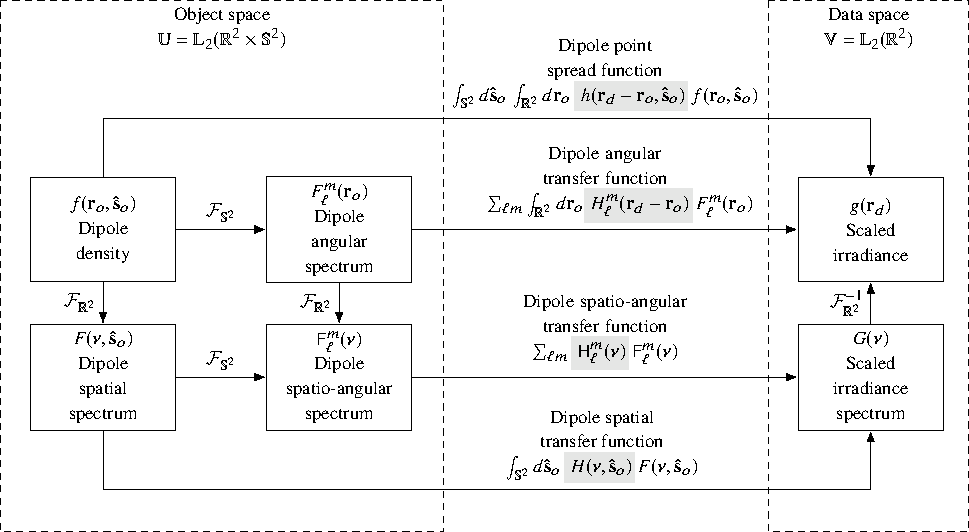
\includegraphics[scale=1.0]{../figures/dipole-block/dipole-block.pdf}
  \caption{We can compute the mapping between object space and data space using
    four different bases.}
   \label{fig:dipole-block}      
    \end{figure}

\subsection{Paraxial epi-fluorescence microscope}\label{sec:para}
\tb{This section is probably the most mature, but it still has some mismatch with
  newer sections. I've quit using ``kernel'' and haven't fixed it.}
In this section we apply the tools we developed in the previous two sections to
analyze a paraxial epi-fluorescence microscope. We start by reviewing the
derivation of the monopole point spread function in preparation for the
derivation of the orientation-dependent point spread function. We conclude the
section by analyzing the dipole imaging map in the four bases we described
earlier.

\subsubsection{Monopole point spread function}
In this section we derive the form of the monopole point spread function $h(\mb{r})$.
First, we place a monopole emitter at the focal point of an objective lens and
calculate the field created in the back focal plane. We can model a paraxial
thin lens as a quadratic phase element, so it converts a spherical wave to a
plane wave in the back focal plane with a sharp cutoff at the exit pupil of the
lens
\begin{align}
  U_{\text{bfp}}(\mb{r}_b) \propto \Pi\left(\frac{|\mb{r}_b|}{\alpha}\right) \equiv
  \begin{cases}
    1\quad \text{if}\quad |\mb{r}_b| < \alpha,\\
    0\quad \text{else}.
  \end{cases}
\end{align}
A central result of Fourier optics is that the fields one focal distance from
either side of a paraxial lens are related by a scaled two-dimensional Fourier
transform. If we place a detector in the focal plane of the tube lens then the
field on the detector is given by
\begin{align}
  U_{\text{det}}(\mb{r}_d) \propto \mc{F}_{\mbb{R}^2}\left\{U_{\text{bfp}}(\mb{r}_b)\right\} = \frac{J_1(k\alpha|\mb{r}_d|)}{k\alpha|\mb{r}_d|}.
\end{align}
Finally, the detector measures the irradiance instead of the field, so we take
the modulus squared of the field to find that the measurable irradiance created
by a single monopole radiator at the origin is the familiar Airy disk
\begin{align}
  h(\mb{r}_d, \ro = 0) \propto |U_{\text{det}}(\mb{r}_d)|^2 = \left[\frac{J_1(k\alpha|\mb{r}_d|)}{k\alpha|\mb{r}_d|}\right]^2.
\end{align}
Shifting the monopole in the transverse plane will introduce a linear phase
factor in the back focal plane which will manifest as a shift on the detector
due to the Fourier shift theorem. Therefore, the monopole imaging system is
shift invariant and we can rewrite the irradiance on the detector due to a
monopole at $\ro$ as
\begin{align}
  h(\rd, \ro) = h(\rd - \ro). \label{eq:shift}
\end{align}
We have modeled a microscope with unit magnification, but a similar point spread
function can be found for magnifying microscopes by making a change of
variables---see Barrett section 7.2.7.

Rotating a monopole will leave its image unchanged. Therefore, our imaging
system is rotation invariant and we can simplify the orientation-dependent point spread function further with
\begin{align}
  h(\rd - \ro) = h(|\rd - \ro|). \label{eq:rotational}
\end{align}

\subsubsection{Orientation-dependent point spread function}
In the next two subsections we will calculate the orientation dependent point
spread function $h(\mb{r}, \mh{s})$ of a paraxial epi-fluroescence microscope.
We can make our first simplifying step by realizing the excitation and detection
processes are incoherent which means that the orientation-dependent PSF is
separable
\begin{align}
  h(\rd, \ro, \so) = h_{\text{exc}}(\ro, \so)\,h_{\text{det}}(\rd, \ro, \so). \label{eq:kernelsep}
\end{align}
We can calculate the excitation and detection PSFs separately then take their product to find the complete orientation-dependent PSF. 

\subsubsection{Dipole excitation model}
When we developed the monopole imaging model we ignored the excitation process
because we excited the fluorophores with a spatially uniform excitation beam and
monopoles have no orientation dependence. For the dipole imaging model we must
model the excitation process because the excitation process is rarely angularly
uniform (carefully calibrated TIRF systems are an exception).

In this section we will calculate the excitation kernel
$h_{\text{exc}}(\ro, \so)$ for the paraxial epi-illumination microscope under
unpolarized K\"{o}ehler illumination shown in Figure \ref{fig:microscope}. We
will only consider spatially uniform excitation, so the excitation kernel will
no depend on $\ro$
\begin{align}
  h_{\text{exc}}(\ro, \so) = h_{\text{exc}}(\so).
\end{align}
We can interpret $h_{\text{exc}}(\so)$ as the relative probability of exciting a
molecule with dipole orientation $\so$. Our approach is similar to previous work
\cite{fourkas2001, chandler2017}, but here we consider paraxial, incoherent, and
unpolarized illumination.

\begin{figure}[h]
 \centering
   \centering
   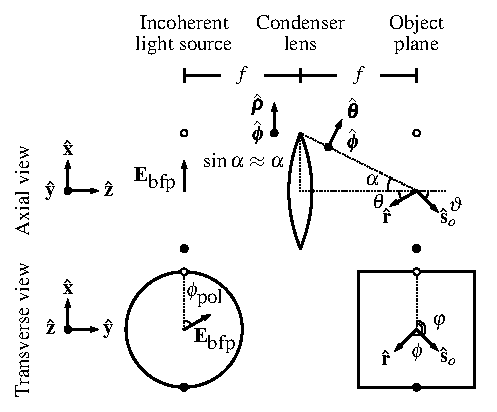
\includegraphics[scale=.9]{../figures/excitation-coords/excitation-coords.pdf}
   \caption{Illumination geometry and coordinates. We calculate the excitation
     kernel $h_{\text{exc}}(\so)$ for a paraxial, unpolarized, incoherent
     light source (or its image) in the back focal plane of the condenser lens. }
   \label{fig:microscope}
 \end{figure}

We start by expressing the dipole moment $\so{}$ in Cartesian coordinates
\begin{align}
  \so{} &= s_x\mh{x} + s_y\mh{y} + s_z\mh{z}. \label{eq:spherical}
\end{align}
We place the dipole in the focal plane of an aplanatic and
polarization-preserving objective lens with its optical axis aligned with the
$\mh{z}$ axis. Next, we place a spatially incoherent, spatially uniform,
unpolarized light source (or its image) in the back aperture of the objective
lens to illuminate the focal plane. In this geometry each point in the back
focal plane generates a plane wave that illuminates the sample.

To model the unpolarized light source we will use polarized ray tracing
\cite{foreman2011} to find the response for a single polarized ray, then
integrate over the rays and polarizations to find the complete response. First,
we model the electric field at every point on the back focal plane as
\begin{align}
   \mb{E}_{\text{bfp}}(\phi_{\text{pol}}) &\propto \cos\phi_{\text{pol}}\mh{x} + \sin\phi_{\text{pol}}\mh{y}, \label{eq:bfp0}
\end{align}
where $\phi_{\text{pol}}$ is the polarization orientation and \{$\mh{x}$,
$\mh{y}$\} are transverse Cartesian basis vectors. Note that Eq. \ref{eq:bfp0}
describes the incoherent electric fields at every point in the back focal
plane--- it does not describe a coherent plane wave. To find the electric field
immediately after the paraxial lens we apply a position-dependent rotation
matrix (see the rotation matrices in \cite{foreman2011, backer2014} under the
paraxial approximation)

\begin{align}
  \mb{E}_{\text{ff}}(\theta, \phi, \phi_{\text{pol}}) & \propto 
  \begin{bmatrix}
    1 & 0 &\theta \cos\phi\\
    0 & 1 &\theta \sin\phi\\
    -\theta\cos\phi&-\theta \sin(\phi)&1
  \end{bmatrix}
  \begin{bmatrix}
    \cos\phi_{\text{pol}}\\
    \sin\phi_{\text{pol}}\\
    0
  \end{bmatrix}\\
  \mb{E}_{\text{ff}}(\theta, \phi, \phi_{\text{pol}}) &\propto \cos\phi_{\text{pol}}\mh{x} + \sin\phi_{\text{pol}}\mh{y} - \theta\cos(\phi - \phi_{\text{pol}})\mh{z}.\label{eq:eff}
\end{align}
The probability that a dipole oriented along $\so{}$ is excited by a ray with
electric field $\mb{E}$ is given by 
\begin{align}
  |\mb{E}_{\text{ff}}(\theta, \phi, \phi_{\text{pol}}) \cdot \so{}|^2 \propto s_x^2\cos^2\phi_{\text{pol}} + s_y^2\sin^2\phi_{\text{pol}} + s_z^2\theta^2\cos^2(\phi - \phi_{\text{pol}}). \label{eq:integrand}
\end{align}
To find the complete excitation kernel we need to integrate Eq.
\ref{eq:integrand} over all polarization orientations and rays
\begin{align}
  h_{\text{exc}}(\so{}) \propto \int_0^{\alpha}\theta d\theta\int_0^{2\pi}d\phi\int_0^{2\pi}d\phi_{\text{pol}}\, |\mb{E}_{\text{ff}}(\theta, \phi, \phi_{\text{pol}}) \cdot \so{}|^2, \label{eq:integral}
\end{align}
where $\alpha$ is the maximum angle the illumination rays make with the optical
axis. Plugging Eq. \ref{eq:integrand} into Eq. \ref{eq:integral}, evaluating the
integrals, and dropping constants gives
\begin{align}
  h_{\text{exc}}(\vartheta) &\propto s_x^2 + s_y^2 + \frac{1}{2}\alpha^2s_z^2.
\end{align}
We can rewrite the excitation kernel in terms of a single variable with the
substitutions $s_x^2 + s_y^2 = \sin^2\vartheta$ and $s_z^2 = \cos^2\vartheta$
\begin{align}
  h_{\text{exc}}(\vartheta) &\propto \sin^2\vartheta + \frac{1}{2}\alpha^2\cos^2\vartheta \label{eq:hexctheta}.
\end{align}

Figure \ref{fig:excitation} shows the excitation kernel as a function of
inclination angle $\vartheta$ and maximum excitation angle $\alpha$. The largest
variation of the excitation kernel occurs when the maximum excitation angle is
zero---plane-wave illumination. As $\alpha$ grows dipoles parallel to the optic
axis are more likely to be excited and the variation of the excitation kernel
decreases. Note that we have derived this simple model under the paraxial
approximation, so it does not make quantitative predictions for high-NA
illumination geometries.
\begin{figure}[h]
 \centering
   \centering
   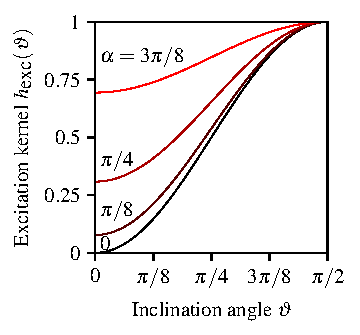
\includegraphics[scale=0.95]{../figures/excitation/excitation.pdf}
   \caption{Dipole excitation kernel $h_{\text{exc}}(\vartheta)$ as a function of
     inclination angle $\vartheta$ and maximum excitation angle $\alpha$.}
   \label{fig:excitation}
 \end{figure}

 \subsubsection{Dipole detection model}
 In this section we will calculate the detection kernel of an epi-detection
 microscope---the irradiance on the detector due to a single dipole with fixed
 position and orientation. Our approach mimics existing work \cite{backer2014,
   nov2006, agrawal2012}, but we restrict ourselves to the paraxial
 approximation.

\begin{figure}[h]
 \centering
   \centering
   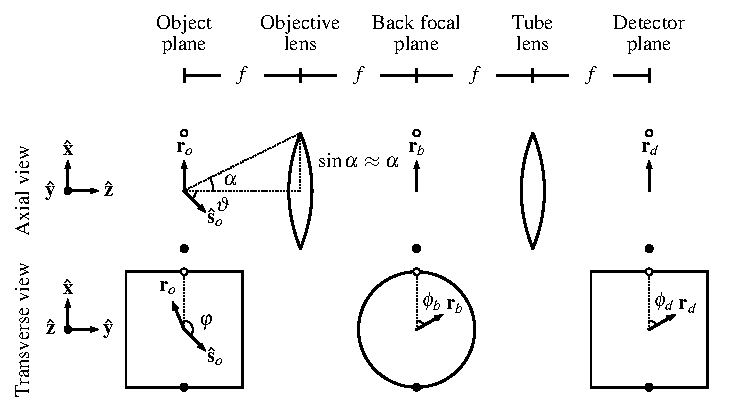
\includegraphics[scale=.9]{../figures/detection-coords/detection-coords.pdf}
   \caption{Detection geometry and coordinates. We calculate the detection
     kernel $h_{\text{det}}(\rd, \ro, \so)$ for a paraxial 4$f$ imaging
     system.}
   \label{fig:detection}
 \end{figure}
 
We consider a single dipole emitter at the origin with a fixed dipole emission
moment oriented along $\so{}$. The electric field at a position $\mb{r}$ far
from the dipole is given by
\begin{align}
  \mb{E}_{\text{ff}}(\mb{r}, \so{}) \propto \frac{\text{exp}[ik|\mh{r}|]}{|\mh{r}|}\mh{r} \times \so{} \times \mh{r}. \label{eq:ff}
\end{align}
We place the dipole in the focal plane of the same 4$f$ imaging system we
considered in the monopole case---see Figure \ref{fig:detection}. The dipole emits
spherical wavefronts so we can reuse our argument for shift invariance and drop
the phase dependence of the electric field
\begin{align}
  \mb{E}_{\text{ff}}(\mb{r}, \so{}) \propto \mh{r} \times \so{} \times \mh{r} \label{eq:ff2}
\end{align}
We also note that we can rewrite a shift-invariant kernel as
\begin{align}
h_{\text{det}}(\rd, \ro, \so) = h_{\text{det}}(\rd - \ro, \so), 
\end{align}
which will simplify our derivation---we only need to calculate the response for
a dipole positioned along the optic axis. We can rewrite the cross products in terms
of a matrix multiplication
\begin{align}
  \mb{E}_{\text{ff}}(\mb{r}, \so{}) \propto [\mb{I} - \mh{r}\mh{r}^{\dagger}]\so,
\end{align}
where $\mb{I}$ is a $3\times 3$ identity matrix. If we place the molecule in the
focal plane of an aplanatic and polarization-preserving objective lens with its
optical axis aligned with the $\mh{z}$ axis (or reuse the illumination
objective), then we can find the electric field in the back focal plane by
multiplying the electric field with a position-dependent rotation matrix and
truncating waves outside the detection collection angle $\alpha$
\begin{align}
  \mb{E}_{\text{bfp}}(\mb{r}, \so{}) \propto \mb{R}_{\text{obj}}(\mh{r})[\mb{I} - \mh{r}\mh{r}^{\dagger}]\so\Pi\left(\frac{\theta}{\alpha}\right).
\end{align}
After plugging in paraxial positions
\begin{align}
  \mh{r}(\theta,\phi) \approx \theta\cos\phi\mh{x} + \theta\sin\phi\mh{y} + \mh{z},
\end{align}
and the paraxial rotation matrix
\begin{align}
  \mb{R}_{\text{obj}}(\theta, \phi) &=
  \begin{bmatrix}
    1 & 0 &-\theta \cos\phi\\
    0 & 1 &-\theta \sin\phi\\
    -\theta\cos\phi&-\theta \sin(\phi)&1
  \end{bmatrix},
\end{align}
then dropping the $\theta^2$ $\mh{z}$ components and changing from spherical
coordinates to cylindrical coordinates by substituting $(r_b, \phi_b)$ for
$(\theta, \phi)$ we find that
\begin{align}
  \mb{E}_{\text{bfp}}(r_b, \phi_b, \so{}) \propto \left\{\left[s_x - s_zr_b\cos\phi_b\right]\mh{x} + \left[s_y - s_z r_b\sin\phi_b\right]\mh{y}\right\}\Pi\left(\frac{r_b}{\alpha}\right). \label{eq:bfp2}
\end{align}
Equation \ref{eq:bfp2} is easier to work with if we introduce the radial vector
field $\mh{\bs{\rho}} = \cos\phi_b\mh{x} + \sin\phi_b\mh{y}$ and rewrite as
\begin{align}
  \mb{E}_{\text{bfp}}(r_b, \phi_b, \so{}) \propto \left\{s_x\mh{x} + s_y\mh{y} - s_z r_b \mh{\bs{\rho}}\right\}\Pi\left(\frac{r_b}{\alpha}\right). \label{eq:bfp3}
\end{align}
Equation \ref{eq:bfp3} shows that the transverse components of the dipole
($s_x, s_y$) create linear vector fields in the back focal plane
($\mh{x}, \mh{y}$) while the axial component of the dipole $s_z$ creates a radial
vector field in the back focal plane $\mh{z}$. 

We complete the 4$f$ system by placing a tube lens one focal length from the
back focal plane and a planar detector---see Figure \ref{fig:detection}. Under
the paraxial approximation we can find the electric field in the detector plane
by taking the Fourier transform of the field in the back focal plane
\cite{goodman1996}
\begin{align}
  \mb{E}_{\text{det}}(\rd{}, \so{}) &= \int_{\mbb{R}^2}d\rb{} \mb{E}_{\text{bfp}}(\rb{})\, \text{exp}\left[ik\,\rb{}\cdot\rd{}\right].\label{eq:det1}
\end{align}
We evaluate the integral in Appendix \ref{sec:ftvec} and show that 
\begin{align}
  \mb{E}_{\text{det}}(r_d, \so{}) \propto \frac{J_1(k\alpha r_d)}{k\alpha r_d}s_x\mh{x} + \frac{J_1(k\alpha r_d)}{k\alpha r_d}s_y\mh{y} - i\alpha\frac{J_2(k\alpha r_d)}{k\alpha r_d}s_z\mh{\bs{\rho}}.
\end{align}
Once again we find that the transverse component of the dipole creates a linear
field and the axial component of the dipole creates a radial field, but on the
detector the linear and radial fields are out of phase by $\pi/2$. This crucial
phase factor is a direct consequence of the fact that the linear fields are real
and even---the Fourier transform of a real and even function is real and
even---and the radial fields are real and odd---the Fourier transform of a real
and odd function is imaginary and odd.

Our final step is to calculate the irradiance on the detector
\begin{align}
  h_{\text{det}}(r_d, \so{}) &\propto |\mb{E}_{\text{det}}(r_d, \so{})|^2.
\end{align}
The irradiance is the sum of the contributions from the linear and radial fields
since their fields are out of phase, so
\begin{align}
  h_{\text{det}}(r_d, \vartheta) &\propto a_1(r_d)\sin^2\vartheta + \frac{1}{2}\alpha^2 a_2(r_d)\cos^2\vartheta, 
\end{align}
where we have defined
\begin{align}
  a_n(r_d) \equiv \frac{n}{\pi}\left[\frac{J_n(k\alpha r_d)}{k\alpha r_d}\right]^2. 
\end{align}
Notice that we retain the $\alpha^2$ irradiance term even though we dropped
$\theta^2$ electric field terms since these terms would become $\theta^2$
irradiance terms.

Figures \ref{fig:hdet} and \ref{fig:microscope} summarize the most important
features of the dipole detection model. When $\alpha$ is very small the
detection kernel is the usual Airy pattern weighted by $\sin^2\vartheta$. Note
that the monopole detection model ignores the $\sin^2\vartheta$ dependence---see
Figure \ref{fig:microscope} a) and b). As $\alpha$ grows the relative
contribution of the higher-order Airy pattern increases. The most important
result is that the dipole detection model is not separable into the product of
a spatial and angular kernel---even under the paraxial approximation. The detection
model is only separable when $\alpha$ approaches zero which is almost never the
case in real microscopes. We refer to the non-separability of the detection
kernel as \textit{spatio-angular coupling} because the orientation of the dipole
is coupled to the spatial pattern of irradiance on the detector.

The paraxial detection kernel is rotationally symmetric---it depends on $r_d$ instead of
$\rd$. This symmetry is a result of the $\pi/2$ phase shift between the linear
and radial fields on the detector. If the phase shift between the linear and
radial fields was not exactly $\pi/2$ then the fields would interfere on the
detector, and we would lose rotational symmetry. Tracing back further, the
rotational symmetry is due to the fact that the field in the back focal plane
could be written as a sum of a linear and radial field which is only true under
the paraxial approximation---the rotational symmetry of the detection kernel is
only true to first order. Despite the approximation, we still feel that the
rotational symmetry of the detection kernel is a valuable result since it helps
build an intuition about the dominant effects outside the paraxial
approximation. Later in this work we will exploit this approximate symmetry to
improve the efficiency of simulating and inverting the imaging model. 

Note that we have restricted our analysis to an imaging system with unit
magnification. We will continue with this simplification and mention that an
imaging system with an arbitrary magnification can be modeled using the model
for a system with unit magnification and a change of variable (see
\cite{barrett2004} section 7.2.7).

\begin{figure}[h]
 \centering
   \centering
   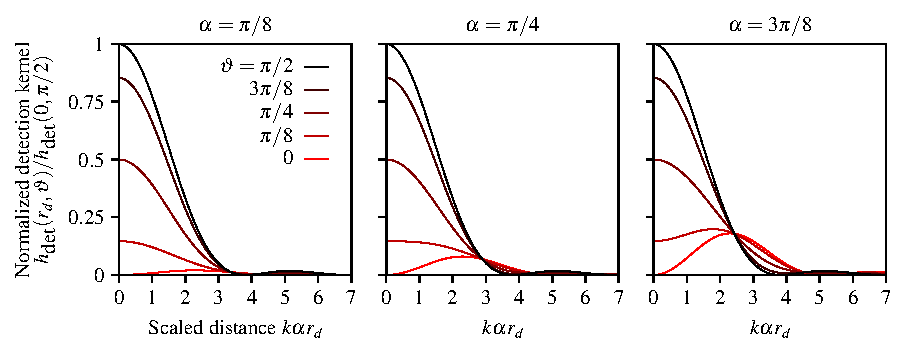
\includegraphics[scale=0.8]{../figures/detection/detection.pdf}
   \caption{Normalized detection kernel as a function of the scaled radial
     detection coordinate $k\alpha r_d$, the dipole inclination angle
     $\vartheta$, and the collection angle $\alpha$. For small
     collection angles (left) the detection kernel of axial dipoles
     (\textcolor{red}{\textbf{red}}) is small compared to transverse dipoles
     (\textbf{black}), but the relative contribution of axial dipoles increases
     with the collection angle (see \textcolor{red}{\textbf{red}} lines from
     left to right).}
   \label{fig:hdet}
 \end{figure}
 
\begin{figure}[h]
 % \captionsetup{width=1.0\linewidth}
 \centering
   \centering
   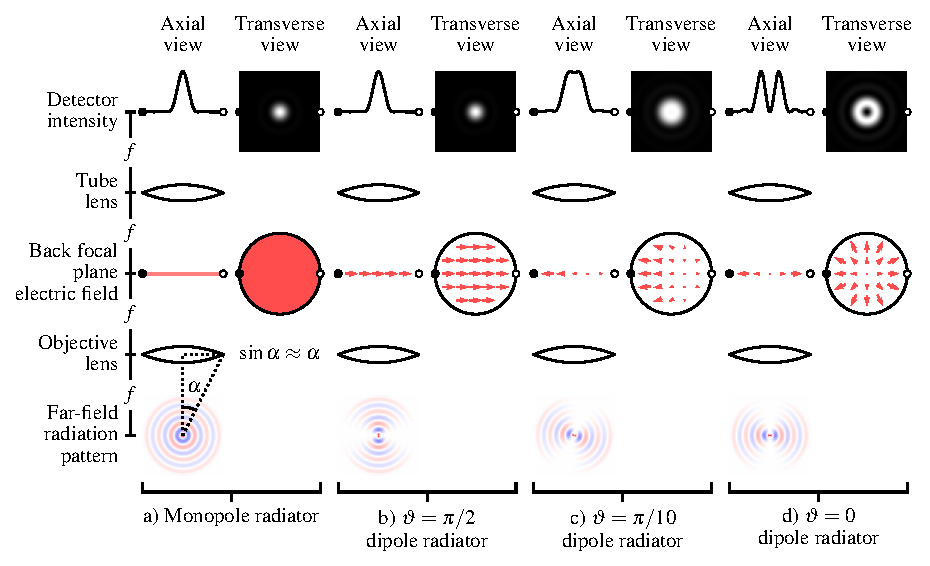
\includegraphics[scale=0.8]{../figures/microscope/microscope.pdf}
   \caption{Comparison of paraxial detection models for monopole radiators a)
     and dipole radiators b)--d). a) Monopole radiators fill the back focal
     plane with a uniform scalar field which gives rise to the familiar Airy
     disk on the detector. b) A transverse dipole radiator also creates an Airy
     disk, but the back focal plane is filled with a uniform vector field. c) An
     axial dipole radiator creates a radial electric field pattern in the back
     focal plane which creates a higher-order Airy disk on the detector. d)
     Dipoles that are not transverse or axial still create radially symmetric
     irradiance patterns under the paraxial approximation. Fields from
     transverse dipoles are real and even while fields from axial dipoles are
     real and odd which causes a relative $\pi/2$ phase shift for the fields on
     the detector. This phase shift means that the fields from transverse and
     axial components of the dipole do not interfere which causes radially
     symmetric irradiance patterns.}
   \label{fig:microscope}
 \end{figure}

 \subsubsection{Simplified dipole imaging model}
 Combining the results of the previous two sections yields a simplified dipole
 imaging model 
 \begin{align}
g(\rd{}) = \int_{\mbb{S}^2}d\so{}\int_{\mbb{R}^2}d\ro{}\, h(|\rd - \ro|, |\so\cdot \mh{z}|)f(\ro, \so).\label{eq:simplified}
 \end{align}
 where we have written the kernel in terms of $|\so\cdot\mh{z}| = \cos\vartheta$
 to explicitly show the dependence on $\so$. In previous sections we showed that the
 kernel is given by 
 \begin{align}
   h(r, \vartheta) &\propto h_{\text{exc}}(\vartheta)h_{\text{det}}(r,\vartheta).
 \end{align}
 Plugging in our results
 \begin{align}
   h(r, \vartheta) &\propto \left[\sin^2\vartheta + \frac{1}{2}\alpha^2 \cos^2\vartheta\right]\left[a_1(r)\sin^2\vartheta + \frac{1}{2}\alpha^2 a_2(r)\cos^2\vartheta\right]. \label{eq:sa-psf}
 \end{align}

 \subsubsection{Orientation-dependent optical transfer function}\label{sec:trans}
  In Appendix \ref{sec:airy} we evaluate the 2D spatial Fourier transforms of
  $a_1(r)$ and $a_2(r)$ to find that
  \begin{align}
    H(\nu, \vartheta) &\propto \left[\sin^2\vartheta + \frac{1}{2}\alpha^2 \cos^2\vartheta\right]\left[A_1(\nu)\sin^2\vartheta + \frac{1}{2}\alpha^2 A_2(\nu)\cos^2\vartheta\right].
  \end{align}
  where 
\begin{align}
  A_1(\nu) &= \frac{2}{\pi}\left\{\cos^{-1}\left(\frac{\nu}{2\nu_o}\right) - \frac{\nu}{2\nu_o}\sqrt{1 - \left(\frac{\nu}{2\nu_o}\right)^2}\right\}\Pi\left(\frac{\nu}{2\nu_o}\right), \\
  A_2(\nu) &= \frac{2}{\pi}\Bigg\{\cos^{-1}\left(\frac{\nu}{2\nu_o}\right) - \left[3 - 2\left(\frac{\nu}{2\nu_o}\right)^2\right]\frac{\nu}{2\nu_o}\sqrt{1 - \left(\frac{\nu}{2\nu_o}\right)^2}\Bigg\}\Pi\left(\frac{\nu}{2\nu_o}\right).
\end{align}
The STF is shown in Figure \ref{fig:odotf}. The STF has the usual
spatial-frequency cutoff at $\nu = 2\nu_o$ for all dipole orientations. 

\begin{figure}[h]
 % \captionsetup{width=1.0\linewidth}
 \centering
   \centering
   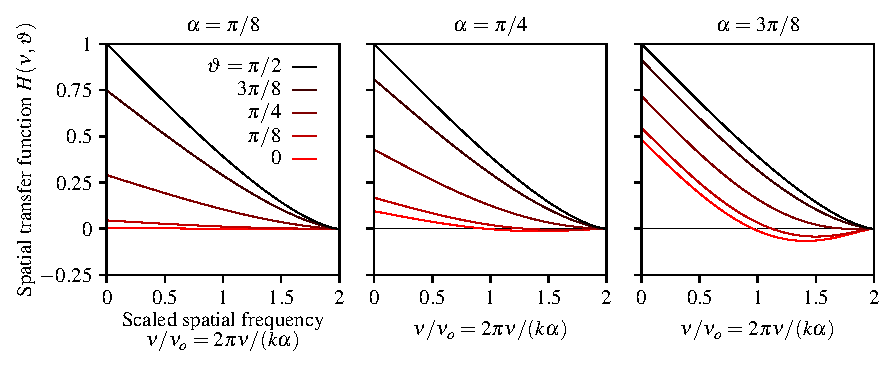
\includegraphics[scale=0.8]{../figures/stf/stf.pdf}
   \caption{STF as a function of the scaled spatial frequency, the dipole
     inclination angle $\vartheta$, and the collection angle $\alpha$. For small
     collection angles (left) the STF for axial dipoles
     (\textcolor{red}{\textbf{red}}) is small compared to transverse dipoles
     (\textbf{black}), but the relative contribution of axial dipoles increases
     with the collection angle (see \textcolor{red}{\textbf{red}} lines from
     left to right). The STF of axial dipoles is negative at high spatial
     frequencies because the central minimum of the axial kernel corresponds to
     the position of the dipole. Equivalently, a high-spatial-frequency pattern
     of axial dipoles will generate an irradiance pattern where the minimum
     irradiance corresponds to the peak of the axial dipole density.}
   \label{fig:odotf}
 \end{figure}

\subsubsection{Angular transfer function (ATF)}

To calculate the angular transfer function we plug the spatio-angular point
spread function Eq. \ref{eq:sa-psf} into Eq. \ref{eq:atf-prep} and evaluate the
integrals using a computer algebra package \cite{meurer2017} to find
\begin{alignat}{6}
  H_l^m(r) \propto \quad 7&\{\hphantom{-}32&&a_1(r)&& + 4\alpha^2[a_1(r) + a_2(r)]&&+ 3\alpha^4a_2(r)\}&&\delta_{\ell 0}\delta_{m0}+\nonumber\\
  4\sqrt{5}&\{-16&&a_1(r)&& + \hphantom{1}\alpha^2[a_1(r) + a_2(r)] &&+ 3\alpha^4a_2(r)\}&&\delta_{\ell 2}\delta_{m0} + \nonumber\\
  8&\{\hphantom{-1}4&&a_1(r)&& - 2\alpha^2[a_1(r) + a_2(r)] &&+ \hphantom{1}\alpha^4a_2(r)\}&&\delta_{\ell 4}\delta_{m0}.
\end{alignat}
The degree $\ell$ and order $m$ of the non-zero terms in the ATF follow directly
from specific features of the kernel. First, our kernel is symmetric under
inversion of the dipole moment which appears in the kernel as even-degreed
trigonometric functions. This symmetry is maintained in the ATF since all of the
non-zero terms have an even degree $\ell=0, 2$, and $4$. Second, we showed that
under the paraxial approximation our kernel is rotationally symmetric which
allows us to write the kernel as a function of $r$ instead of $\mb{r}$. This
symmetry is maintained in the ATF since all of the non-zero terms have order
$m=0$. Finally, both the excitation and detection kernels are a weighted sum of
degree-2 trigonometric functions which implies that the maximum degree of the
kernel is 4. This feature of the kernel appears in the ATF since only
$\ell=0, 2$, and $4$ terms are non-zero. 

\begin{figure}[h]
 \centering
   \centering
   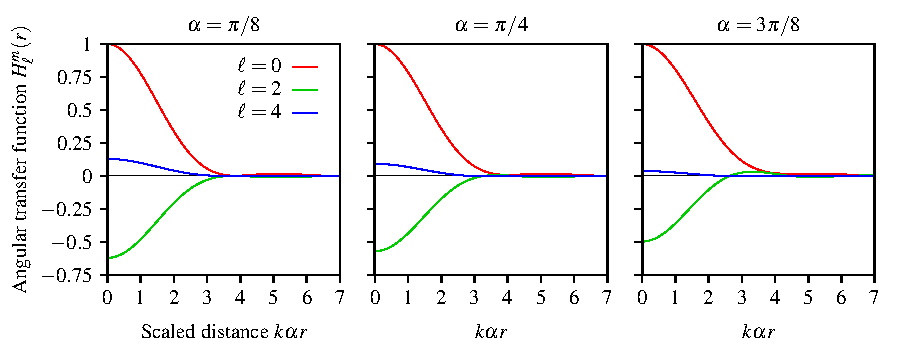
\includegraphics[scale=0.8]{../figures/atf/atf.pdf}
   \caption{ATF as a function of the scaled radial detection coordinate
     $k\alpha r$, the spherical harmonic degree $\ell$, and the collection angle
     $\alpha$. 
   }
   \label{fig:atf}
 \end{figure}


 \subsubsection{Spatio-angular transfer function (SATF)}
  \begin{alignat}{6}
  H_l^m(\nu) \propto \quad 7&\{\hphantom{-}32&&A_1(\nu)&& + 4\alpha^2[A_1(\nu) + A_2(\nu)]&&+ 3\alpha^4A_2(\nu)\}&&\delta_{\ell 0}\delta_{m0}+\nonumber\\
  4\sqrt{5}&\{-16&&A_1(\nu)&& + \hphantom{1}\alpha^2[A_1(\nu) + A_2(\nu)] &&+ 3\alpha^4A_2(\nu)\}&&\delta_{\ell 2}\delta_{m0} + \nonumber\\
  8&\{\hphantom{-1}4&&A_1(\nu)&& - 2\alpha^2[A_1(\nu) + A_2(\nu)] &&+ \hphantom{1}\alpha^4A_2(\nu)\}&&\delta_{\ell 4}\delta_{m0}.
\end{alignat}

\begin{figure}[h]
 \centering
   \centering
   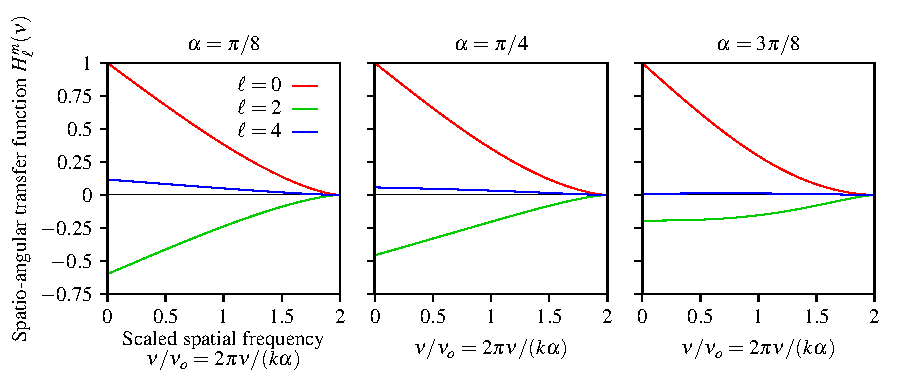
\includegraphics[scale=0.8]{../figures/satf/satf.pdf}
   \caption{SATF as a function of the scaled spatial frequency, the spherical
     harmonic degree $\ell$, and the collection angle $\alpha$. }
   \label{fig:atf}
 \end{figure}
 
\section{Results}
\subsection{Phantom with spatio-angular sparsity (single molecules)}
\subsection{Phantom with spatial sparsity (rotating single molecules)}
\subsection{Phantom with angular sparsity (actin fibers)}
\subsection{Phantom without sparsity (most general)} 

\section{Discussion \tb{Very rough but open for discussion}}
\subsection{Reconstructions}
Since the ATF effectively contains three OTFs it is tempting to conclude that
fluorescence microscopes pass three times as much information about the dipoles
as monopoles. This is not true. The microscope still only measures a single
member of $\mbb{L}_2(\mbb{R}^2)$ so at best we can recover the same amount of
information about the object. In other words, we know immediately that the
microscope is a rank-1 operator since it only measures one continuous function.

We postpone a full discussion of SVD to find the object space singular functions
that span the measurement space of the instrument.

\subsection{Alternative transfer functions}
Throughout this work we have used the spherical harmonic functions as a basis
for functions on the sphere, but there are other basis functions that can be
advantageous in some cases. Backer and others [CITE TODO] have used the second
moments as basis functions for the sphere because they arise naturally when
computing the spatio-angular point spread function. Mathematically, Backer and
Lew use an alternative to the angular transfer function that uses the second
moments as basis functions so their forward model is given by
\begin{align}
  g(\rd) = \sum_{j=1}^6 H_j(\rd - \ro)F_j(\ro)
\end{align}
where
\begin{align}
  H_j(\rd - \ro) &= \int_{\mbb{S}^2}d\so\, h(\rd - \ro, \so)Z_j(\so),\\
  F_j(\ro) &= \int_{\mbb{S}^2}d\so\, f(\ro, \so)Z_j(\so),
\end{align}
and $Z_j(\mh{s}) = \{s_x^2, s_y^2, s_z^2, s_xs_y, s_ys_z, s_xs_z\}$ are the
second moments. This formulation provides the main advantage of the ATF
approach---efficient computation for spatially sparse and angularly dense
samples---without requiring a cumbersome expansion of the spatio-angular point
spread function onto spherical harmonics.

The spherical harmonics provide several advantages over the second moments as
well. First, the spherical harmonics form an orthonormal basis which often
simplifies computation. For example, if we calculated the angular detection
transfer function we would find that it contained two angular terms under the
paraxial approximation. If we expanded onto second moments we would need all six
angular basis functions and computing the forward model would be three times as
expensive. Second, the spherical harmonics are complete which means they can
represent arbitrary functions on the sphere while the second moments can only
represent a small subset of all functions on the sphere. Extending the accuracy
of the second moments using the fourth (or higher) moments is possible, but it
requires a completely new basis. Indeed, the simple microscope we consider in
this work requires an expansion onto fourth-order spherical harmonics, so an
expansion onto second-order moments would not suffice. Finally, using the
spherical harmonics provides access to a set of fast algorithms. The naive
expansion of an arbitrary discretized $N$ point spherical function onto
spherical harmonics (or second moments) requires a $\mc{O}(N^2)$ matrix
multiplication while pioneering work by Driscoll and Healy [cite] showed that the
forward discrete fast spherical harmonic transform can be computed with a
$\mc{O}(N(\log N)^2)$ algorithm and its inverse can be computed with a
$\mc{O}(N^{3/2})$ algorithm. To our knowledge no similarly fast algorithms exist
for expansion onto the higher-order moments.

The diffusion magnetic resonance imaging uses both sets of bases [cite Basser]
[cite Tournier] for particular cases. 

\subsection{What determines the angular frequency cutoff?}
The spatial-frequency cutoff of a fluorescence microscope is well known to vary
as NA$/\lambda$---we can increase spatial resolution by increasing the NA of the
instrument or by choosing a fluorophore with a shorter emission wavelength.
Analogously, the angular-frequency spectrum of a fluorescence microscope depends
on both the instrument and the sample.

The simple paraxial microscope considered in this work always has three terms in
its angular-frequency spectrum, but we can increase the number of terms by
modifying the instrument. We will postpone the proper treatment of these effects
until future work, but we briefly mention that the number of terms in the
angular-frequency spectrum increases for non-paraxial microscopes, microscopes
with polarizers on the illumination or detection paths, and multiview
microscopes. We also mention that there are two ways to extend the
angular-frequency spectrum of a microscope---by increasing the degree $\ell$ and
by increasing the order $m$. Extending the angular degree cutoff $\ell_0$ gives
the microscope the ability to measure finer angular features, while extending
the angular order cutoff $m_0$ give the microscope the ability to measure
features of the object that are increasingly invariant to rotation. If the
angular order cutoff matches the angular degree cutoff $\ell_0 = m_0$ then the
microscope can be said to have $\textit{isotropic angular resolution}$. This
condition is not met by a single-view paraxial microscope since $\ell_0 = 4$ and
$m_0 = 0$, but we will model microscopes with this property in future work. 

The number of terms in the angular frequency spectrum is also sample dependent.
Monopoles emit light isotropically so they have a single term, dipoles have a
three-term ATF, and higher-order excitation and detection moments will have even
more terms---these objects have different angular band limits. We emphasize the
similarity between the spatial and angular frequency cutoffs---both the sample
and the instrument affect the maximum achievable resolution of the imaging
system.

Possibly implies that the spatio-angular transfer function can be factored. Cite
3D vector transfer functions Arnison and Sheppard.  

\subsection{Characterizing real spatio-angular microscopes}
The theoretical model we present in this work is an extreme simplification of a
real microscope. We have ignored the effects of thick samples, optical
aberration, scattering, high-NA objectives, finite fluorescence lifetimes, and
interactions between fluorophores, and we are sure that this list of limitations
could be extended. Because of this long list of unknown effects, real
experiments should make an attempt to characterize the specific imaging system.

Typical fluorescence microscopy experiments start with the monopole
approximation and attempt to characterize the microscope by imaging
sub-diffraction beads. These images are assumed to be good approximations of the
monopole point spread function and this data can be used to restore (deconvolve)
the data taken in arbitrary experiments.

Imaging sub-diffraction beads is not enough to completely characterize the
response of a microscope to a an oriented sample. We need at least three samples
with a known orientations to characterize the SATF, so isotropic beads are not
enough. Small beads may not be isotropic [cite Lew]. 

\section{Conclusion}
Most models of fluorescence microscopes use a monopole model to describe the
object and the imaging system. A more complete description of any fluorescence
microscope requires a dipole model of the object and a model of the
spatio-angular point spread function. We developed several transfer functions
that simplify the mapping between the spatio-angular density and the irradiance
pattern on the detector, and we demonstrated these transfer functions by
efficiently simulating a paraxial widefield fluorescence microscope.



\bibliography{paper}
\appendix
\section{Fourier transform of linear and radial vector fields}\label{sec:ftvec}
  \begin{align}
  \mb{E}_{\text{det}}(\rd{}, \so{}) &= \int_{\mbb{R}^2}d\rb{} \mb{E}_{\text{bfp}}(\rb{})\, \text{exp}\left[ik\,\rb{}\cdot\rd{}\right].\label{eq:det1}
\end{align}
To evaluate the integral we rewrite it in polar coordinates
\begin{align}
\mb{E}_{\text{det}}(\rd{}, \so{}) &= \int_{0}^{\alpha}r_bdr_b\int_0^{2\pi} d\phi_b\, \mb{E}_{\text{bfp}}(r_b, \phi_b)\, \text{exp}\left[ikr_b r_d\cos(\phi_b - \phi_d)\right],
\end{align}
plug in Eq. \ref{eq:bfp2}, and apply the following identities
\begin{align}
  \int_0^{2\pi}d\phi_b
  \left\{\substack{
    \sin(n\phi_b)\\
    \cos(n\phi_b)
  }\right\}
  \text{exp}\left[ikr_br_d\cos(\phi_b - \phi_d)\right] &= 2\pi i^n
  \left\{\substack{
    \sin(n\phi'_o)\\
    \cos(n\phi'_o)
  }\right\}J_n(k r_br_d),
  \end{align}
  \begin{align}
  \int_0^{\alpha} dr_b (r_b)^{n+1}J_{n}(kr_br_d) &= \alpha^{n+1}\left[\frac{J_{n+1}(k\alpha r_d)}{k r_d}\right],
  \end{align}
to find that 
\begin{align}
  \mb{E}_{\text{det}}(\rd{}, \so{}) \propto &\left[s_x\frac{J_1(k\alpha r_d)}{k\alpha r_d} - is_z\alpha \frac{J_2(k\alpha r_d)}{k\alpha r_d}\cos\phi_d\right]\mh{x}\, + \nonumber \\& \left[s_y\frac{J_1(k\alpha r_d)}{k\alpha r_d} - i s_z\alpha \frac{J_2(k\alpha r_d)}{k\alpha r_d}\sin\phi_d\right]\mh{y}.
\end{align}
Similar to the back focal plane, we rewrite in terms of linear and radial vector
fields
\begin{align}
  \mb{E}_{\text{det}}(\rd{}, \so{}) \propto \frac{J_1(k\alpha r_d)}{k\alpha r_d}[s_x\mh{x} + s_y\mh{y}] - i\alpha\frac{J_2(k\alpha r_d)}{k\alpha r_d}s_z\mh{\bs{\rho}}.
\end{align}

\section{Spherical harmonics}\label{sec:sph}
% The spherical harmonics are an orthonormal set of basis functions on the sphere.
% In this appendix we will define the basis and review several important
% properties of this set of functions.
The spherical harmonic function of degree $\ell$ and order $-\ell \leq m \leq m$
is defined as \cite{schaeffer2013}
\begin{align}
Y_\ell^m(\vartheta, \varphi) = P_\ell^m\left(\cos\vartheta\right)\exp(i m \varphi)
\end{align}
where $P_\ell^m(\cos\theta)$ are the associated Legendre polynomials normalized for the
spherical harmonics 
\begin{align}
  P_\ell^m(x) = (-1)^m\sqrt{\frac{2\ell+1}{4\pi}}\sqrt{\frac{(\ell-|m|)!}{(\ell+|m|)!}}(1-x^2)^{|m|/2}\frac{d^{|m|}}{dx^{|m|}}P_\ell(x)
\end{align}
where $P_\ell(x)$ are the Legendre polynomials defined by the following recurrence
\begin{align}
  P_0(x) &= 1,\\
  P_1(x) &= x,\\
  \ell P_\ell(x) &= (2\ell-1)xP_{\ell-1}(x) - (\ell-1)P_{\ell-2}(x). 
\end{align}

The spherical harmonics are orthonormal which means that
\begin{align}
  \int_{\mbb{S}^2}d\mh{s}\, Y_\ell^m(\mh{s})\bar{Y}_{\ell'}^{m'}(\mh{s}) = \delta_{\ell\ell'}\delta_{mm'},
\end{align}
where $\delta_{\ell\ell'}$ denotes the Kronecker delta. The spherical harmonics form a
complete basis so an arbitrary function on the sphere $f(\mh{s})$ can be
expanded into a sum of weighted spherical harmonic functions
\begin{align}
  f(\mh{s}) = \sum_{\ell=0}^{\infty}\sum_{m=-\ell}^{l}F_\ell^mY_\ell^m(\mh{s}).
\end{align}
We can find the spherical harmonic coefficients $F_\ell^m$ for a given function by
using Fourier's trick---multiply both sides by $\bar{Y}_\ell^m(\mh{s})$, integrate
over the sphere, and exploit orthogonality to find that
\begin{align}
  F_\ell^m = \int_{\mbb{S}^2}d\mh{s}\, f(\mh{s})\bar{Y}_\ell^m(\mh{s}).
\end{align}
The coefficients $F_\ell^m$ are usually called the \textit{spherical Fourier
  transform} of a spherical function.

We briefly show how two properties of spherical functions propagate to the
spherical Fourier transform. First, the spherical harmonic coefficients of
spherical functions that can be written entirely as a function of the
inclination angle $\vartheta$ are zero when $m\neq0$ because
\begin{align}
  \int_{\mbb{S}^2}d\mh{s}\, f(\vartheta)\bar{Y}_\ell^m(\mh{s}) &= \int_0^{2\pi}d\phi\, \text{exp}[-im\varphi]\int_0^{\pi}d\vartheta\, \sin\vartheta f(\vartheta)P_\ell^m(\cos\vartheta),\\ &= \delta_{m0}\int_0^{\pi}d\vartheta\, \sin\vartheta f(\vartheta)P_\ell^m(\cos\vartheta).
\end{align}
Second, the spherical harmonic coefficients of spherical functions that are
symmetric under inversion $f(\mh{s}) = f(-\mh{s})$ are zero when $\ell$ is odd
because $Y_\ell^m(-\so) = (-1)^\ell Y_\ell^m(\mh{s})$, so if $\ell$ is odd then
\begin{align}
  \int_{\mbb{S}^2}d\mh{s}\, f(\mh{s})\bar{Y}_{2n+1}^m(\mh{s}) &= \int_{\mbb{S}^2/2}d\mh{s}\, f(+\mh{s})\bar{Y}_{2n+1}^m(+\mh{s}) + \int_{\mbb{S}^2/2}d\mh{s}\, f(-\mh{s})\bar{Y}_{2n+1}^m(-\mh{s}),\\
&=\int_{\mbb{S}^2/2}d\mh{s}\, f(\mh{s})\bar{Y}_{2n+1}^m(+\mh{s}) - \int_{\mbb{S}^2/2}d\mh{s}\, f(\mh{s})\bar{Y}_{2n+1}^m(\mh{s}) = 0.                                                                
\end{align}
\section{Fourier transform of first and second order Airy patterns} \label{sec:airy}
\begin{align}
    a_n(r_d) \equiv \frac{n}{\pi}\left[\frac{J_n(k\alpha r_d)}{k\alpha r_d}\right]^2. 
\end{align}
\begin{align}
  A_n(\nu) \equiv \mathcal{F}_2\{a_n(r_o)\} =  \int_{\mbb{R}^2}d\ro{}\,\text{exp}\left[i2\pi \ro{}\cdot\bs{\nu}\right] a_n(r_d), \label{eq:ftA}
\end{align}

Our final task is to calculate $A_1(\nu)$ and $A_2(\nu)$. $A_1(\nu)$ is a
well-known result \cite{goodman1996, mertz2009}, but we review the calculation
to establish the tools we'll need to evaluate $A_2(\nu)$. We start by using the
autocorrelation (Wiener-Khinchin) theorem to rewrite the Fourier transform as
\begin{align}
  A_1(\nu) = \frac{1}{\pi}\mathcal{F}_2\left\{\left[\frac{J_1(2\pi\nu_o r_o)}{2\pi\nu_o r_o}\right]^2\right\} = \frac{1}{\pi}\left[\mathcal{F}_2\left\{\frac{J_1(2\pi\nu_o r_o)}{2\pi\nu_o r_o}\right\} \star_2 \mathcal{F}_2\left\{\frac{J_1(2\pi\nu_o r_o)}{2\pi\nu_o r_o}\right\}\right] \label{eq:auto}
\end{align}
where $\star_2$ denotes a two-dimensional autocorrelation. Next, we recognize
that the Fourier transforms on the right hand side of Eq. \ref{eq:auto} are
rotationally symmetric so they can be rewritten as zero-order Hankel transforms
\begin{align}
  A_1(\nu) = \frac{1}{\pi}\left[\mathcal{H}_0\left\{\frac{J_1(2\pi\nu_o r_o)}{2\pi\nu_o r_o}\right\} \star_2 \mathcal{H}_0\left\{\frac{J_1(2\pi\nu_o r_o)}{2\pi\nu_o r_o}\right\}\right] \label{eq:autoz}
\end{align}
We can apply the Hankel transform identity \cite{poul1998}
\begin{align}
  \mathcal{H}_{n-1}\left\{\frac{J_n(2\pi\nu_o r_o)}{2\pi\nu_o r_o}\right\} = \frac{\nu^{n-1}}{\nu_o^{n}}\Pi\left(\frac{\nu}{\nu_o}\right),\label{eq:identity}
\end{align}
to find that 
\begin{align}
  A_1(\nu) = \frac{1}{\pi\nu_o^{2}}\left[\Pi\left(\frac{\nu}{\nu_o}\right) \star_2 \Pi\left(\frac{\nu}{\nu_o}\right)\right] \label{eq:auto3}. 
\end{align}
We can use the geometric construction in Figure \ref{fig:geometry} to express the
autocorrelation in terms of an integral over a region of overlap between
two circles given by
\begin{align}
  A_1(\nu) &= \frac{4}{\pi\nu_o^{2}}\left[\int_0^{\nu_o}\tau d\tau\int_0^{\cos^{-1}\left(\frac{\nu}{2\nu_o}\right)}d\phi_{\tau} - \int_{0}^{\nu/2}d\tau_x\int_0^{\tau_x\frac{2\nu_o}{\nu}\sqrt{1 - \left(\frac{\nu}{2\nu_o}\right)^2}}d\tau_y\right]\Pi\left(\frac{\nu}{2\nu_o}\right),\\
  A_1(\nu) &= \frac{4}{\pi\nu_o^{2}}\left[\int_0^{\nu_o}\tau d\tau\cos^{-1}\left(\frac{\nu}{2\nu_o}\right) - \int_{0}^{\nu/2}d\tau_x\tau_x\frac{2\nu_o}{\nu}\sqrt{1 - \left(\frac{\nu}{2\nu_o}\right)^2}\right]\Pi\left(\frac{\nu}{2\nu_o}\right),\\
  A_1(\nu) &= \frac{2}{\pi}\left\{\cos^{-1}\left(\frac{\nu}{2\nu_o}\right) - \frac{\nu}{2\nu_o}\sqrt{1 - \left(\frac{\nu}{2\nu_o}\right)^2}\right\}\Pi\left(\frac{\nu}{2\nu_o}\right).
\end{align}
\begin{figure}[h]
 % \captionsetup{width=1.0\linewidth}
 \centering
   \centering
   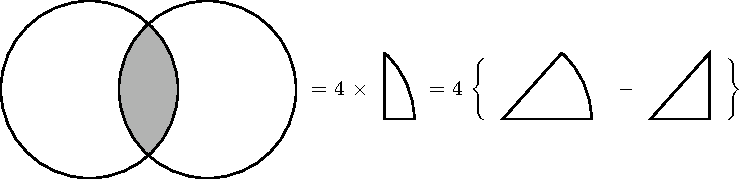
\includegraphics[width = 0.8\textwidth]{../figures/autocorrelation/autocorrelation.pdf}
   \caption{Geometric construction for evaluating the autocorrelations. We need
     to integrate over the overlapping region of two circles with radius $\nu_o$
     and distance $\nu$ between their centers. The region is given by four times
     the difference in area between a sector of angle
     $\arccos\left(\frac{\nu}{2\nu_o}\right)$ and a triangle with base $\nu/2$
     and hypotenuse $\nu_o$.}
   \label{fig:geometry}
 \end{figure}

 To evaluate $A_2(\nu)$ we could follow the same steps, but we will reach a dead
 end because there is no Hankel transform identity for
 $\mathcal{H}_{n-1}\left\{\frac{J_{n+1}(2\pi\nu_o r_o)}{2\pi\nu_o r_o}\right\}$.
 Instead, we rewrite $A_2(\nu)$ as
\begin{align}
  A_2(\nu) = \frac{2}{\pi}\mathcal{F}_2\left\{\left[\frac{J_2(2\pi\nu_o r_o)}{2\pi\nu_o r_o}\right]^2\right\} = \frac{2}{\pi}\left[\mathcal{F}_2\left\{\left[\frac{J_2(2\pi\nu_o r_o)}{2\pi\nu_o r_o}\cos\phi_{\nu}\right]^2\right\} + \mathcal{F}_2\left\{\left[\frac{J_2(2\pi\nu_o r_o)}{2\pi\nu_o r_o}\sin\phi_{\nu}\right]^2\right\}\right].
\end{align}
Applying the autocorrelation theorem gives
\begin{align}
  A_2(\nu) = \frac{2}{\pi}\Bigg[&\mathcal{F}_2\left\{\frac{J_2(2\pi\nu_o r_o)}{2\pi\nu_o r_o}\cos\phi_{\nu}\right\} \star_2 \mathcal{F}_2\left\{\frac{J_2(2\pi\nu_o r_o)}{2\pi\nu_o r_o}\cos\phi_{\nu}\right\} + \nonumber\\ &\mathcal{F}_2\left\{\frac{J_2(2\pi\nu_o r_o)}{2\pi\nu_o r_o}\sin\phi_{\nu}\right\} \star_2 \mathcal{F}_2\left\{\frac{J_2(2\pi\nu_o r_o)}{2\pi\nu_o r_o}\sin\phi_{\nu}\right\}\Bigg].
\end{align}
After converting the Fourier transforms to Hankel transforms with the identities
\begin{align}
  \mathcal{F}_2\left\{f(r)\cos(\phi)\right\} &= -i\cos\phi_{\nu}\mathcal{H}_1\left\{f(r)\right\},\\
  \mathcal{F}_2\left\{f(r)\sin(\phi)\right\} &= -i\sin\phi_{\nu}\mathcal{H}_1\left\{f(r)\right\},
\end{align}
and evaluating the Hankel transforms with Eq. \ref{eq:identity}, we find that
\begin{align}
  A_2(\nu) = -\frac{2}{\pi\nu_o^4}\left\{\left[\nu_x\Pi\left(\frac{\nu}{\nu_o}\right) \star_2 \nu_x\Pi\left(\frac{\nu}{\nu_o}\right)\right] + \left[\nu_y\Pi\left(\frac{\nu}{\nu_o}\right) \star_2 \nu_y\Pi\left(\frac{\nu}{\nu_o}\right)\right]\right\}. \label{eq:long}
\end{align}
Eq. \ref{eq:long} contains two autocorrelations that require us to find the
weighted overlap of two circles. Neither of these autocorrelations are
rotationally symmetric, but their sum must be rotationally symmetric. With this
symmetry in mind, we recognize that the first autocorrelation is largest for
shifts along the $x$ direction and smallest for shifts along the $y$ direction
with a smooth $\cos^2\phi_{\nu}$ weighting between the two extremes. The same is
true for the second autocorrelations except the $x$ and $y$ axes are exchanged
and there is a $\sin^2\phi_{\nu}$ weighting between the two extremes. Therefore,
we can rewrite Eq. \ref{eq:long} as
\begin{align}
  A_2(\nu) = -\frac{2}{\pi\nu_o^4}\Bigg\{&\left[\nu_x\Pi\left(\frac{\nu}{\nu_o}\right) \star_2^x \nu_x\Pi\left(\frac{\nu}{\nu_o}\right)\right]\cos^2\phi_\nu + \left[\nu_x\Pi\left(\frac{\nu}{\nu_o}\right) \star_2^y \nu_x\Pi\left(\frac{\nu}{\nu_o}\right)\right]\sin^2\phi_\nu + \nonumber\\ &\left[\nu_y\Pi\left(\frac{\nu}{\nu_o}\right) \star_2^x \nu_y\Pi\left(\frac{\nu}{\nu_o}\right)\right]\cos^2\phi_\nu + \left[\nu_y\Pi\left(\frac{\nu}{\nu_o}\right) \star_2^y \nu_y\Pi\left(\frac{\nu}{\nu_o}\right)\right]\sin^2\phi_\nu\Bigg\}. \label{eq:long3}
\end{align}
where $\star_2^x$ denotes a two-dimensional autocorrelation for shifts along
the $x$ direction. We can use the following pair of identities
\begin{align}
  \nu_x\Pi\left(\frac{\nu}{\nu_o}\right) \star_2^x \nu_x\Pi\left(\frac{\nu}{\nu_o}\right) = \nu_y\Pi\left(\frac{\nu}{\nu_o}\right) \star_2^y \nu_y\Pi\left(\frac{\nu}{\nu_o}\right),\\
  \nu_x\Pi\left(\frac{\nu}{\nu_o}\right) \star_2^y \nu_x\Pi\left(\frac{\nu}{\nu_o}\right) = \nu_y\Pi\left(\frac{\nu}{\nu_o}\right) \star_2^x \nu_y\Pi\left(\frac{\nu}{\nu_o}\right),
\end{align}
to simplify Eq. \ref{eq:long3} to
\begin{align}
  A_2(\nu) = -\frac{2}{\pi\nu_o^4}\Bigg\{&\left[\nu_x\Pi\left(\frac{\nu}{\nu_o}\right) \star_2^x \nu_x\Pi\left(\frac{\nu}{\nu_o}\right)\right] + \left[\nu_x\Pi\left(\frac{\nu}{\nu_o}\right) \star_2^y \nu_x\Pi\left(\frac{\nu}{\nu_o}\right)\right]\Bigg\}. \label{eq:long4}
\end{align}
First we evaluate the autocorrelation for shifts along the $x$ axis
\begin{align}
  &= -\frac{2}{\pi\nu_o^4}\left[\nu_x\Pi\left(\frac{\nu}{\nu_o}\right) \star_2^x \nu_x\Pi\left(\frac{\nu}{\nu_o}\right)\right]\\
  &= -\frac{8}{\pi\nu_o^4}\Bigg[\int_0^{\nu_o}\tau d\tau\int_0^{\cos^{-1}\left(\frac{\nu}{2\nu_o}\right)}d\phi_{\tau}(-\tau^2\cos^2\phi_{\tau} + \nu\tau\cos\phi_{\tau})\\ &\hspace{5em}- \int_{0}^{\nu/2}d\tau_x\int_0^{\tau_x\frac{2\nu_o}{\nu}\sqrt{1 - \left(\frac{\nu}{2\nu_o}\right)^2}}d\tau_y(-\tau_x^2 + \nu\tau_x)\Bigg]\Pi\left(\frac{\nu}{2\nu_o}\right).
\end{align}
For the first inner integral we make use of the following identities
\begin{align}
  \int_0^{\cos^{-1}z}d\phi\cos^2\phi &= \frac{1}{2}z\sqrt{1 - z^2} + \frac{1}{2}\cos^{-1}z,\\
  \int_0^{\cos^{-1}z}d\phi\cos\phi &= \sqrt{1 - z^2},
\end{align}
which results in
\begin{align}
  &= -\frac{8}{\pi\nu_o^{4}}\Bigg[\int_0^{\nu_o}d\tau\frac{-\tau^3}{2}\left(\frac{\nu}{2\nu_o}\sqrt{1 - \left(\frac{\nu}{2\nu_o}\right)^2} + \cos^{-1}\left(\frac{\nu}{2\nu_o}\right)\right) + \nu\tau^2\sqrt{1 - \left(\frac{\nu}{2\nu_o}\right)^2}\nonumber\\ &\hspace{5em}\int_{0}^{\nu/2}d\tau_x\int_0^{\tau_x\frac{2\nu_o}{\nu}\sqrt{1 - \left(\frac{\nu}{2\nu_o}\right)^2}}d\tau_y(-\tau_x^2 + \nu\tau_x)\Bigg]\Pi\left(\frac{\nu}{2\nu_o}\right),\\
  &=  -\frac{8}{\pi\nu_o^4}\Bigg[\frac{-\nu_o^4}{8}\left(\frac{\nu}{2\nu_o}\sqrt{1 - \left(\frac{\nu}{2\nu_o}\right)^2} + \arccos\left(\frac{\nu}{2\nu_o}\right) \right) + \frac{2\nu_o^4}{3}\frac{\nu}{2\nu_o}\sqrt{1 - \left(\frac{\nu}{2\nu_o}\right)}\nonumber \\ &\hspace{5em} - \frac{5\nu^2\nu_o^2}{48}\frac{\nu}{2\nu_o}\sqrt{1 - \left(\frac{\nu}{2\nu_o}\right)^2}\Bigg]\Pi\left(\frac{\nu}{2\nu_o}\right),\\
  &=  \frac{1}{\pi}\Bigg[\left(\frac{\nu}{2\nu_o}\sqrt{1 - \left(\frac{\nu}{2\nu_o}\right)^2} + \arccos\left(\frac{\nu}{2\nu_o}\right) \right) - \frac{16}{3}\frac{\nu}{2\nu_o}\sqrt{1 - \left(\frac{\nu}{2\nu_o}\right)}\nonumber \\ &\hspace{5em} + \frac{5\nu^2}{6\nu_o^2}\frac{\nu}{2\nu_o}\sqrt{1 - \left(\frac{\nu}{2\nu_o}\right)^2}\Bigg]\Pi\left(\frac{\nu}{2\nu_o}\right),\\
  &= \frac{1}{\pi}\left[\arccos\left(\frac{\nu}{2\nu_o}\right) - \left(\frac{13}{3} - \frac{5\nu^2}{6\nu_o^2}\right)\frac{\nu}{2\nu_o} \sqrt{1 - \left(\frac{\nu}{2\nu_o}\right)^2}\right]\Pi\left(\frac{\nu}{2\nu_o}\right),\\
  &= \frac{1}{\pi}\left[\arccos\left(\frac{\nu}{2\nu_o}\right) - \frac{1}{3}\left[13 - 10\left(\frac{\nu}{2\nu_o}\right)^2\right]\frac{\nu}{2\nu_o} \sqrt{1 - \left(\frac{\nu}{2\nu_o}\right)^2}\right]\Pi\left(\frac{\nu}{2\nu_o}\right).\label{eq:auto1}
\end{align}
Next we evaluate the autocorrelation for shifts along the $y$ axis
\begin{align}
  &\frac{-2}{\pi\nu_0^4}\left\{\left[\nu_x\, \Pi\left(\frac{\nu}{\nu_o}\right)\right] \star_2^y \left[\nu_x\, \Pi\left(\frac{\nu}{\nu_o}\right)\right]\right\} = \\
  &=  \frac{-8}{\pi\nu_o^4}\Bigg[\int\limits_0^{\nu_o} d\tau\, \tau \int\limits_0^{\cos^{-1}\left(\frac{\nu}{2\nu_o}\right)}d\phi_{\tau}(-\tau^2\sin^2\phi_{\tau}) - \int\limits_0^{\nu/2}d\tau_x \int\limits_0^{\tau_x \frac{2\nu_o}{\nu}\sqrt{1 - \left(\frac{\nu}{2\nu_o}\right)^2}}d\tau_y(-\tau_y^2)\Bigg]\Pi\left(\frac{\nu}{2\nu_o}\right).
\end{align}
For the first inner integral we make use of
\begin{align}
  \int\limits_0^{\cos^{-1}z} d\phi \sin^2\phi &= -\frac{1}{2}z\sqrt{1 - z^2} + \frac{1}{2}\cos^{-1}(z).
\end{align}
This results in
\begin{align}
  &=\frac{-8}{\pi\nu_o^4}\Bigg[\int\limits_0^{\nu_o} d\tau\, \frac{-\tau^3}{2}\left(\frac{-\nu}{2\nu_o}\sqrt{1 - \left(\frac{\nu}{2\nu_o}\right)^2} + \cos^{-1}\left(\frac{\nu}{2a}\right)\right) - \int\limits_0^{\nu/2}d\tau_x \frac{-\tau_x^3}{3}\left(\frac{2 \nu_o}{\nu}\sqrt{1 - \left(\frac{\nu}{2\nu_o}\right)^2}\right)^3\Bigg]\Pi\left(\frac{\nu}{2\nu_o}\right),\\
  &=  \frac{-8}{\pi\nu_o^4}\Bigg[\frac{-\nu_o^4}{8}\left(\frac{-\nu}{2\nu_o}\sqrt{1 - \left(\frac{\nu}{2\nu_o}\right)^2} + \cos^{-1}\left(\frac{\nu}{2\nu_o}\right) \right) + \frac{\nu_o^4}{12}\frac{\nu}{2\nu_o}\sqrt[3]{1 - \left(\frac{\nu}{2\nu_o}\right)^2}\Bigg]\Pi\left(\frac{\nu}{2\nu_o}\right),\\
  &=  \frac{1}{\pi}\Bigg[\cos^{-1}\left(\frac{\nu}{2\nu_o}\right) - \frac{1}{3}\left[5 - 2\left(\frac{\nu}{2\nu_o}\right)^2\right]\frac{\nu}{2\nu_o}\sqrt{1 - \left(\frac{\nu}{2\nu_o}\right)^2}\Bigg]\Pi\left(\frac{\nu}{2\nu_o}\right). \label{eq:auto2}
\end{align}
Taking the sum of Eqs. \ref{eq:auto1} and \ref{eq:auto2} gives the final result
\begin{align}
  A_2(\nu) = \frac{2}{\pi}\Bigg\{\cos^{-1}\left(\frac{\nu}{2\nu_o}\right) - \left[3 - 2\left(\frac{\nu}{2\nu_o}\right)^2\right]\frac{\nu}{2\nu_o}\sqrt{1 - \left(\frac{\nu}{2\nu_o}\right)^2}\Bigg\}\Pi\left(\frac{\nu}{2\nu_o}\right). 
\end{align}
% \section{Evaluating the angular transfer function}
% Our goal in this Appendix is to calculate the angular transfer function by
% taking the spherical Fourier transform of
% \begin{align}
%   h(r, \vartheta) = h_{\text{exc}}(\vartheta)h_{\text{det}}(r, \vartheta) &\propto \left[\sin^2\vartheta + \frac{1}{2}\alpha^2 \cos^2\vartheta\right]\left[a_1(r)\sin^2\vartheta + \frac{1}{2}\alpha^2 a_2(r)\cos^2\vartheta.\right] \label{eq:kernel}
% \end{align}
% We need to evaluate the integrals
% \begin{align}
%   F_l^m(r) \propto \int_{\mbb{S}^2} d\so h_{\text{exc}}(\vartheta)h_{\text{det}}(r, \vartheta)Y_\ell^m(\vartheta, \varphi). \label{eq:atf}
% \end{align}
% We could evaluate the integrals in Eq.
% \ref{eq:kernel} using a computer algebra system, but here we evaluate by hand to
% demonstrate a useful trick for taking the spherical harmonic transform of the
% product of two spherical functions. First, we expand both the excitation and
% detection kernels in a sum of spherical harmonic functions
% \begin{align}
%   F_l^m(r) \propto \int_{\mbb{S}^2} d\so \left[\sum_{{\ell'} m'}H_{{\ell'},\text{exc}}^{m'} Y_{\ell'}^{m'}(\vartheta, \varphi)\right]\left[\sum_{{\ell''} m''}H_{{\ell''},\text{det}}^{m''}(r) Y_{\ell''}^{m''}(\vartheta, \varphi)\right]Y_\ell^m(\vartheta, \varphi). 
% \end{align}
% Next, we exchange the order of the sums and integrals
% \begin{align}
%   F_l^m(r) \propto \sum_{\ell' m'}\sum_{\ell'' m''}H_{\ell',\text{exc}}^{m'}H_{\ell'',\text{det}}^{m''}(r) \int_{\mbb{S}^2} d\so Y_\ell^m(\vartheta, \varphi) Y_{\ell'}^{m'}(\vartheta, \varphi) Y_{\ell''}^{m''}(\vartheta, \varphi). 
% \end{align}
% Finally, if we make the definition
% \begin{align}
%   G_{\ell\ell'\ell''}^{mm'm''} = \int_{\mbb{S}^2}d\so\, Y_\ell^m(\vartheta, \varphi) Y_{\ell'}^{m'}(\vartheta, \varphi) Y_{\ell''}^{m''}(\vartheta, \varphi)
% \end{align}
% and write the angular transfer function as
% \begin{align}
%   F_l^m(r) \propto \sum_{\ell' m'}\sum_{\ell'' m''}H_{\ell',\text{exc}}^{m'}H_{\ell'',\text{det}}^{m''}(r) G_{\ell\ell'\ell''}^{mm'm''}. 
% \end{align}
% This is a valuable result because it allows us to compute the spherical harmonic
% transform of the detection and excitation kernels individually then combine the
% results into the final angular transfer function. The constants
% $G_{\ell\ell'\ell''}^{mm'm''}$ are called the \textit{Gaunt coefficients} and
% can be precomputed or found in tables.

% Next, we compute the spherical Fourier transform of the excitation kernel. 
% \begin{align}
%   H_{\ell',\text{exc}}^{m'} \propto \int_{\mbb{S}^2}d\so\, h_{\text{exc}}(\vartheta)Y_{\ell}^m(\vartheta, \varphi). 
% \end{align}
% From Appendix \ref{sec:sph} we know that the integral will be zero except when
% $m=0$ and when $\ell$ is even. Starting with $\ell = 0$ and $m=0$
% \begin{align}
%   H_{0,\text{exc}}^{0} \propto \int_{\mbb{S}^2}d\so\, \left[\sin^2\vartheta + \frac{1}{2}\alpha^2\cos^2\vartheta\right]\left[\frac{1}{\sqrt{4\pi}}\right] = \frac{4\sqrt{\pi}}{3}\left[1 + \frac{\alpha^2}{4}\right].
% \end{align}
% Next we evaluate $\ell = 2$ and $m=0$
% \begin{align}
%   H_{2,\text{exc}}^{0} \propto \int_{\mbb{S}^2}d\so\, \left[\sin^2\vartheta + \frac{1}{2}\alpha^2\cos^2\vartheta\right]\left[\sqrt{\frac{5}{16\pi}}(3\cos^2\vartheta - 1)\right] = \frac{4\sqrt{\pi}}{3}\frac{1}{\sqrt{5}}\left[-1 + \frac{\alpha^2}{2}\right].
% \end{align}
% Finally, we notice can verify that the excitation kernel can be written as just
% two spherical harmonics using the equality
% \begin{align}
%  h_{\text{exc}}(r, \vartheta) &= H_{0,\text{exc}}^0Y_0^0(\vartheta, \varphi) + H_{2,\text{exc}}^0Y_2^0(\vartheta, \varphi),\\
%   \sin^2\vartheta + \frac{1}{2}\alpha^2\cos^2\vartheta &= \frac{4\sqrt{\pi}}{3}\left[1 + \frac{\alpha^2}{4}\right]\left[\frac{1}{\sqrt{4\pi}}\right] + \frac{4\sqrt{\pi}}{3}\frac{1}{\sqrt{5}}\left[-1 + \frac{\alpha^2}{2}\right]\left[\sqrt{\frac{5}{16\pi}}(3\cos^2\vartheta - 1)\right].
% \end{align}

% \begin{align}
%   H_{\ell',\text{exc}}^{m'} \propto \left[1 + \frac{\alpha^2}{4}\right]\delta_{\ell'0}\delta_{m0} + \frac{1}{\sqrt{5}}\left[-1 + \frac{\alpha^2}{4}\right]\delta_{\ell'0}\delta_{m0}.
% \end{align}
% Similarly, the spherical Fourier transform of the detection kernel is given by
% \begin{align}
%   H_{\ell'',\text{det}}^{m''} \propto \left[a_1(r) + \frac{\alpha^2}{4}a_2(r)\right]\delta_{\ell''0}\delta_{m0} + \frac{1}{\sqrt{5}}\left[-a_1(r) + \frac{\alpha^2}{4}a_2(r)\right]\delta_{\ell''0}\delta_{m0}.
% \end{align}
% Finally, we use the Gaunt coefficients to calculate the angular transfer function
% \begin{align}
%   F_l^m(r) \propto \sum_{\ell' m'}\sum_{\ell'' m''}H_{\ell',\text{exc}}^{m'}H_{\ell'',\text{det}}^{m''}(r) G_{\ell\ell'\ell''}^{mm'm''}.   
% \end{align}
% \begin{alignat}{6}
%   F_l^m(r) \propto \quad 7&\{\hphantom{-}32&&a_1(r)&& + 4\alpha^2[a_1(r) + a_2(r)]&&+ 3\alpha^4a_2(r)\}&&\delta_{\ell 0}\delta_{m0}+\nonumber\\
%   4\sqrt{5}&\{-16&&a_1(r)&& + \hphantom{1}\alpha^2[a_1(r) + a_2(r)] &&+ 3\alpha^4a_2(r)\}&&\delta_{\ell 2}\delta_{m0} + \nonumber\\
%   8&\{\hphantom{-1}4&&a_1(r)&& - 2\alpha^2[a_1(r) + a_2(r)] &&+ \hphantom{1}\alpha^4a_2(r)\}&&\delta_{\ell 4}\delta_{m0}.
% \end{alignat}
% H0
% 28*A1*a**2 + 224*A1 + 21*A2*a**4 + 28*A2*a**2
% (Pdb) H2
% 4*sqrt(5)*(A1*a**2 - 16*A1 + 3*A2*a**4 + A2*a**2)
% (Pdb) H4
% -16*A1*a**2 + 32*A1 + 8*A2*a**4 - 16*A2*a**2


\end{document}
